\section{Results}
\label{sec:results}

With our catalog of matched dark matter halos, we are able to directly compare differences in halo properties arising from initialization with \lpt\ vs \za.  We consider halos on a pair--by--pair basis as well as the entire sample as a whole and in different mass bins.  Overall, while we find a fair amount of agreement between \lpt\ and \za\ simulations, we do find an overall trend for \lpt\ halos to be slightly ahead in their time evolution than their \za\ counterparts, specifically in terms of mass, concentration, and relaxation.

We compare halo pairs on an individual halo--by--halo basis by eye for several of the most massive halos.  Morphologies appear to be fairly similar for most halos, indicating good halo matches between simulations.  However, for galaxies undergoing a major merger, the \lpt\ halo mergers appear to often be slightly ``ahead'' of their \za\ counterparts, appearing with a smaller nuclear separation in the case of dual nuclei or even lacking a noticeable second nucleus, while the \za\ merger is still in progress.  For an example halo pair with offset merger epochs, see Figure~\ref{fig:halo-pair}.  The \lpt\ halo seems to be in a nearly post--merger state, with an elongated but singular nucleus, while the \za\ halo has two distinct major components.

\begin{figure}[t]
	\centering
	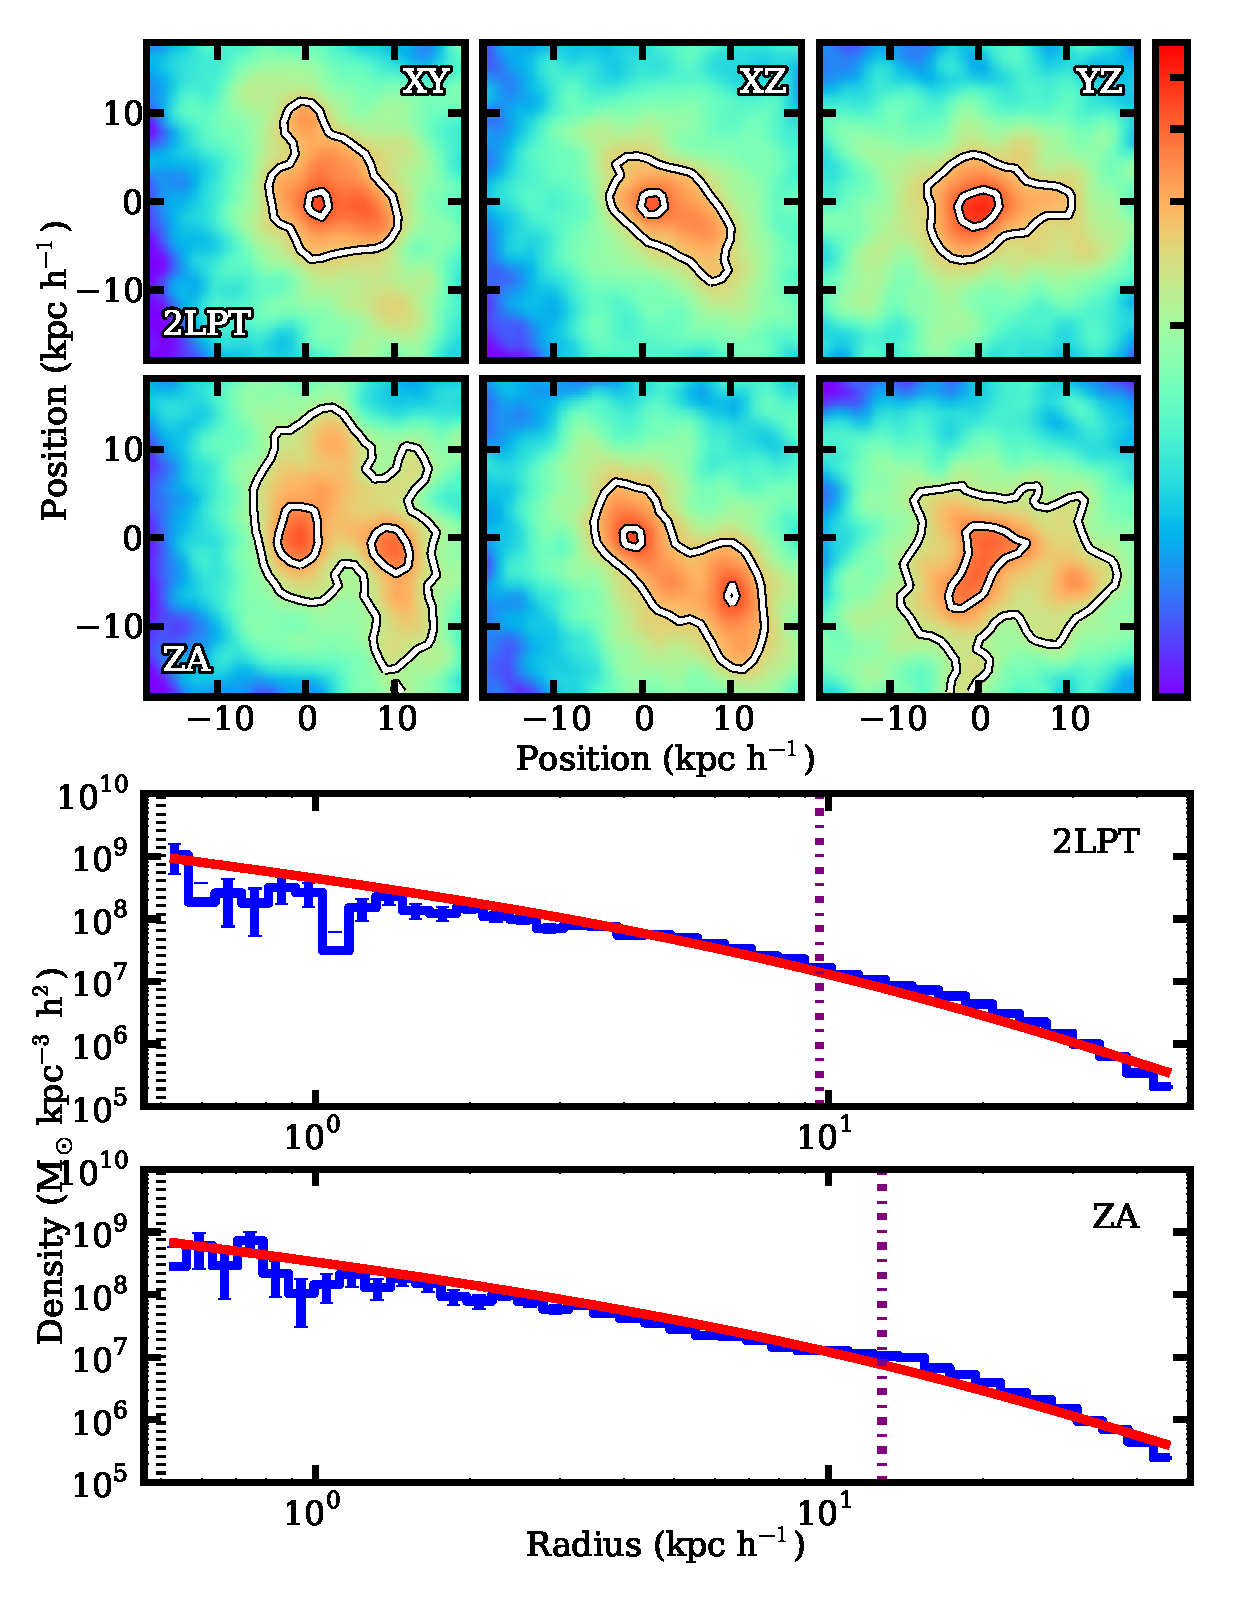
\includegraphics[width=\linewidth]{halo-pair_070_snap061.eps}
	\caption[Comparison of matched \lpt\ and \za\ halos]{\footnotesize \emph{Top two rows:}  \textcolor{red}{Zoom in on nuclei?}  Density projections for two matching halos at $z = 6$.  The first and second row are \lpt\ and \za, respectively.  Each halo is either undergoing or has just undergone a merger.  The \lpt\ halo appears to be further along in the merger process, while the \za\ halo lags behind, still displaying two distinct cores.  \emph{Bottom two rows:}  Density profiles for the same two halos as above.  Logarithmic bins of radial particle position are fit to an NFW profile.  The purple dot--dash line marks the scale radius.  With nearly identical virial radii, the higher concentration of the \lpt\ halo can be seen from its smaller scale radius.  The black dotted line is the resolution limit of the simulations.}
	\label{fig:halo-pair}
\end{figure}

Expanding this to an analysis of the halo population as a whole, we consider consider the central position offset $X_{\mathrm{off}}$, defined as the distance between the halo density peak and the halo center--of--mass \citep{2013ApJ...762..109B}.  In Figure~\ref{fig:diff-hist_Xoff}, we plot histograms of the normalized difference in $X_{\mathrm{off}}$ between halos in the \lpt\ and \za\ simulations
\begin{equation} \label{eq:delta_Xoff}
	\Delta X_{\mathrm{off}} = \frac{X_{\mathrm{off},\lpt} - X_{\mathrm{off},\za}}{X_{\mathrm{off,avg}}}
\end{equation}
for three different redshifts and fit the data with generalized normal distributions also accounting for skew and kurtosis.  Here, and likewise in subsequent histogram fits, we exclude the central bin at $\Delta X_{\mathrm{off}} = 0$ from the fit, measuring only the halo pairs with a non-negligible parameter displacement.  The gray--shaded histogram counts only the halos in the top 25\% mass quartile.  We note that the mean $\Delta X_{\mathrm{off}}$ remains negative throughout the simulations, indicating a consistent trend for \za\ halos to be less relaxed than their \lpt\ counterparts for a given timestep.

\begin{figure}[t]
	\centering
	\begin{subfigure}{}
		\includegraphics[width=\linewidth]{diff-hist_Xoff_snap040_(0.0-1.0).eps}
	\end{subfigure}
	\begin{subfigure}{}
		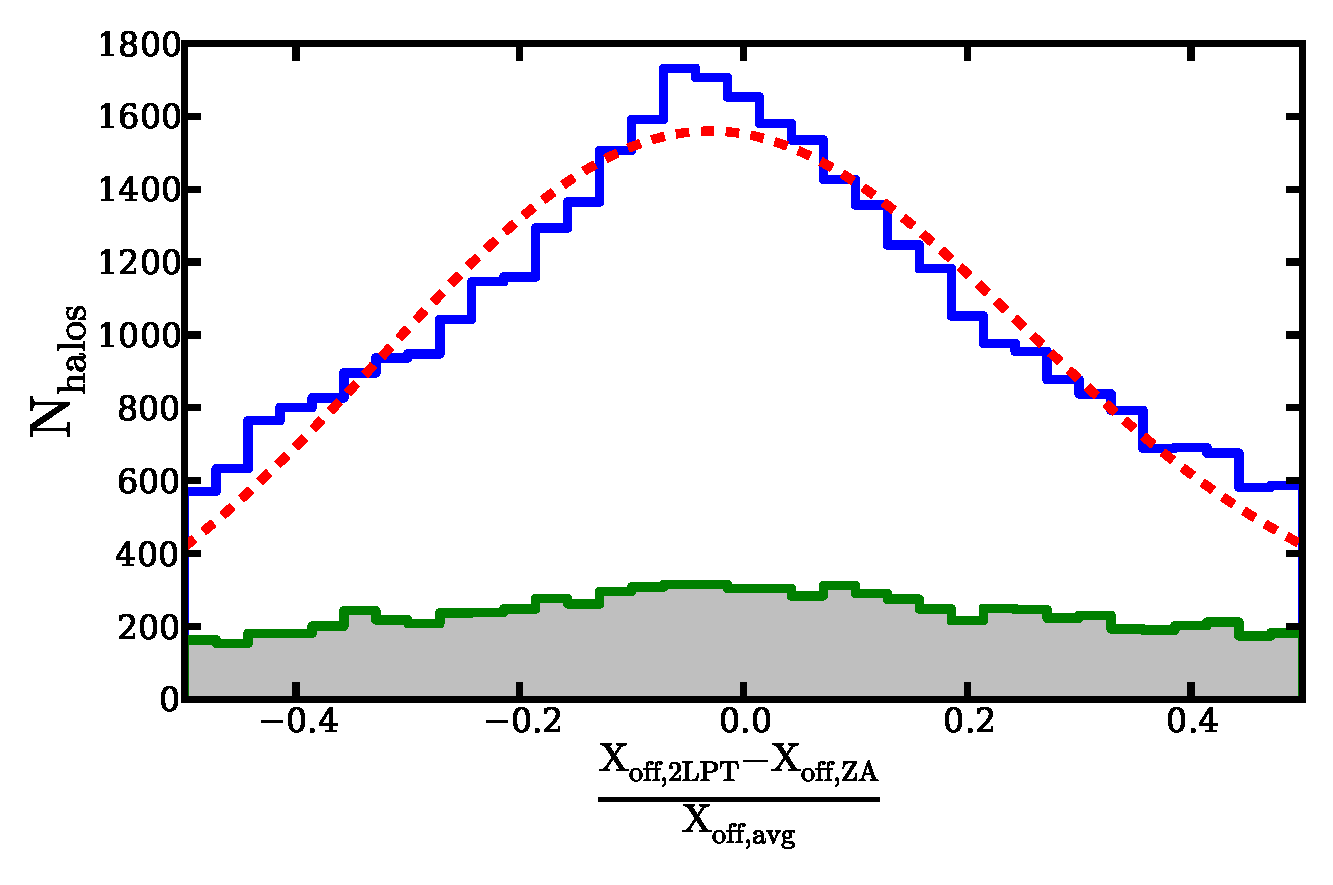
\includegraphics[width=\linewidth]{diff-hist_Xoff_snap050_(0.0-1.0).eps}
	\end{subfigure}
	\begin{subfigure}{}
		\includegraphics[width=\linewidth]{diff-hist_Xoff_snap061_(0.0-1.0).eps}
	\end{subfigure}
	\caption[Histograms of $\Delta X_{\mathrm{off}}$]{\footnotesize Histograms of $\Delta X_{\mathrm{off}}$ for snapshots at $z = 14.7$, $z = 10.3$, and $z = 6.0$ (top, middle, and bottom panels, respectively).  The small gray-filled histograms count only the top 25\% of halos by mass.  The main histograms are fit with a generalized normal distribution accounting for mean, standard deviation, skew, and kurtosis, as shown by the red dashed line.  The central bin at $\Delta X_{\mathrm{off}} = 0$ is ignored for the fit.}
	\label{fig:diff-hist_Xoff}
\end{figure}

In Figure~\ref{fig:diff-hist_Mvir_c}, we plot histograms of the normalized mass difference 
\begin{equation} \label{eq:delta_Mvir}
	\Delta M_{\mathrm{vir}} = \frac{M_{\mathrm{vir},\lpt} - M_{\mathrm{vir},\za}}{M_{\mathrm{vir,avg}}}
\end{equation}
in the left column, and histograms of the normalized concentration difference
\begin{equation} \label{eq:delta_c}
	\Delta c = \frac{c_{\lpt} - c_{\za}}{c_{\mathrm{avg}}}
\end{equation}
in the right column for the same time steps as Figure~\ref{fig:diff-hist_Xoff}.

From a high redshift, we find a tendency for \lpt\ halos to be more massive, with larger halos contributing most to this difference.  The positive mean and skew for the fit data are most evident at high redshift, with a decreasing trend approaching $z = 6$, where the distribution becomes more symmetrical than at higher redshift.  

We see a similar trend for concentration.  As with mass, \lpt\ halos are more concentrated than their \za\ companions, with the largest effect at high redshift.  However, we do not observe the same amount of skew in the distributions at any redshift, and the most massive 25\% of halos are much more evenly distributed about $\Delta c = 0$ than the overall distribution.  We also note that a central peak above the fit curve begins to appear in the histogram, becoming more pronounced toward later redshift, indicating a growing population of halos with little concentration difference between \lpt\ and \za\ simulations.

\begin{figure*}[t]
	\centering
	\begin{subfigure}{}
		\includegraphics[width=0.48\linewidth]{diff-hist_Mvir_snap040_(0.0-1.0).eps}
	\end{subfigure}
	~
	\begin{subfigure}{}
		\includegraphics[width=0.48\linewidth]{diff-hist_c_snap040_(0.0-1.0).eps}
	\end{subfigure}
	\\
	\begin{subfigure}{}
		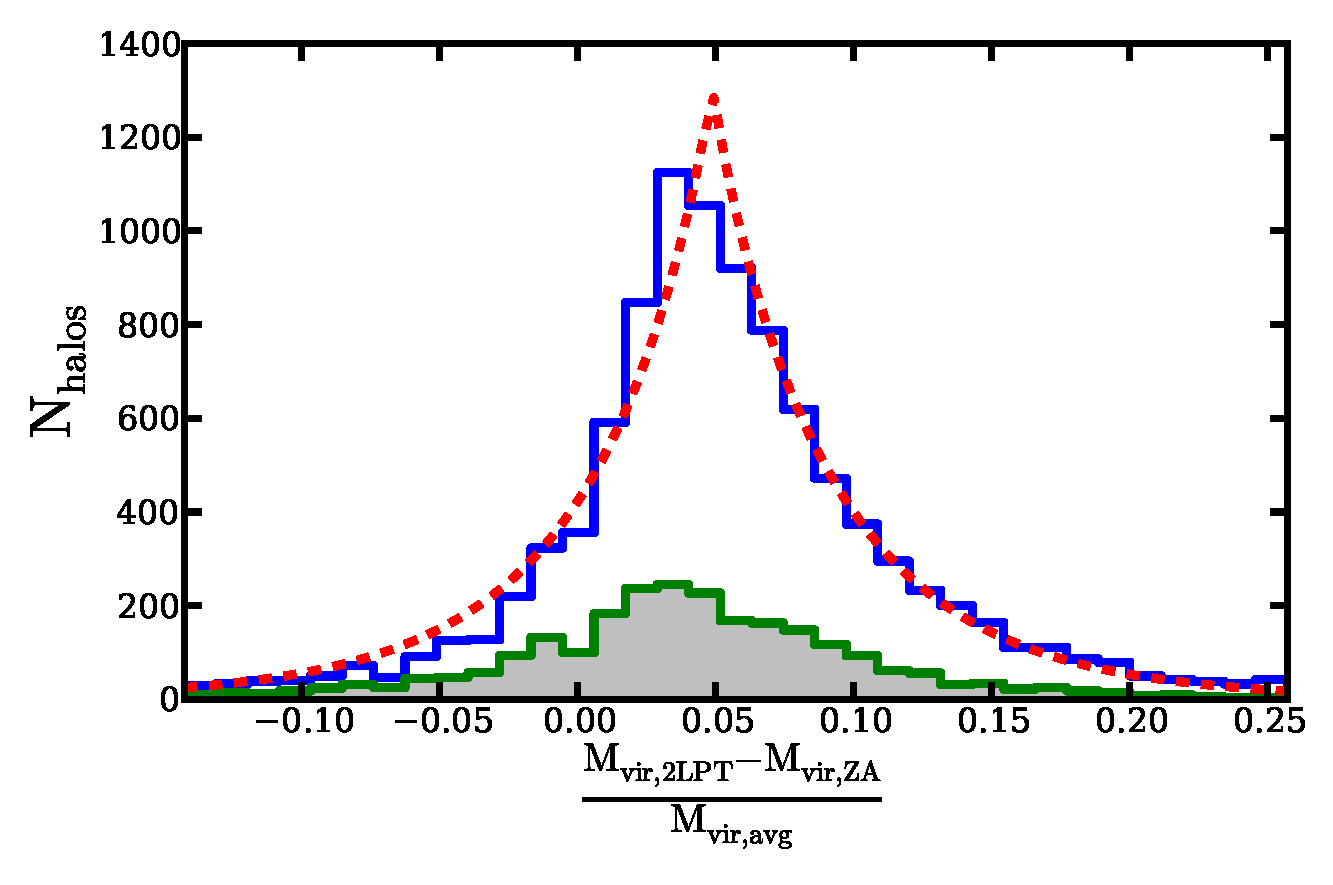
\includegraphics[width=0.48\linewidth]{diff-hist_Mvir_snap050_(0.0-1.0).eps}
	\end{subfigure}
	~
	\begin{subfigure}{}
		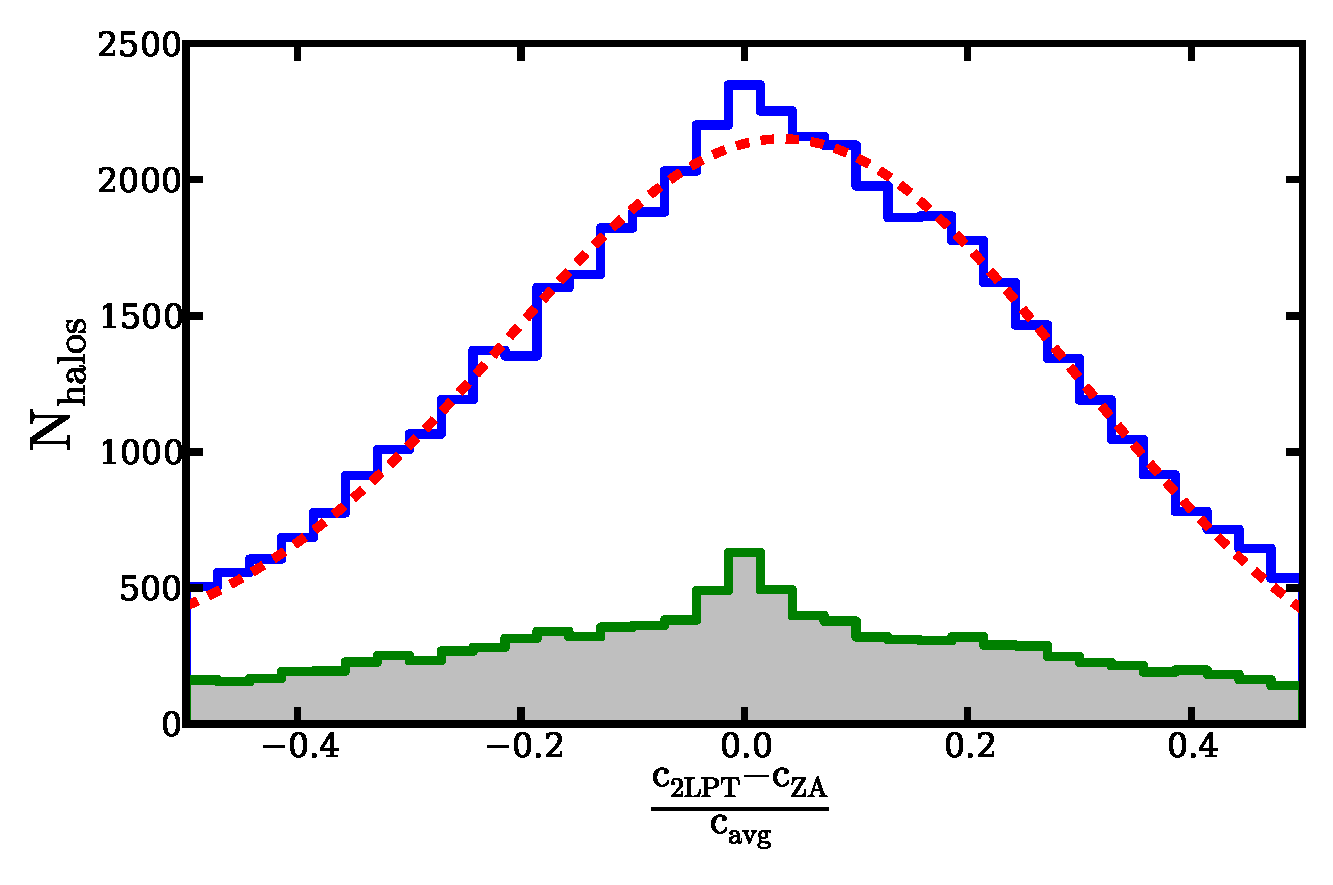
\includegraphics[width=0.48\linewidth]{diff-hist_c_snap050_(0.0-1.0).eps}
	\end{subfigure}
	\\
	\begin{subfigure}{}
		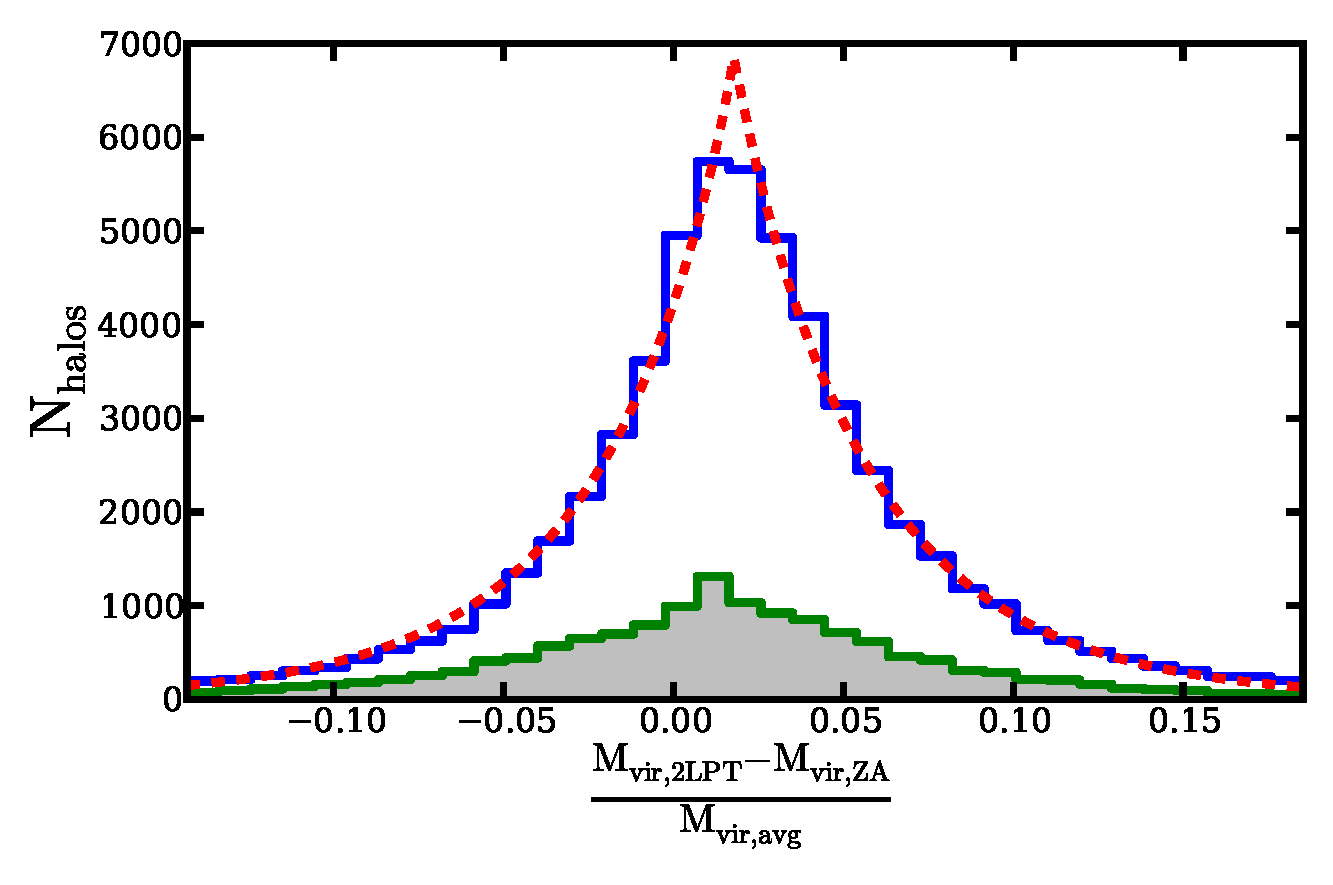
\includegraphics[width=0.48\linewidth]{diff-hist_Mvir_snap061_(0.0-1.0).eps}
	\end{subfigure}
	~
	\begin{subfigure}{}
		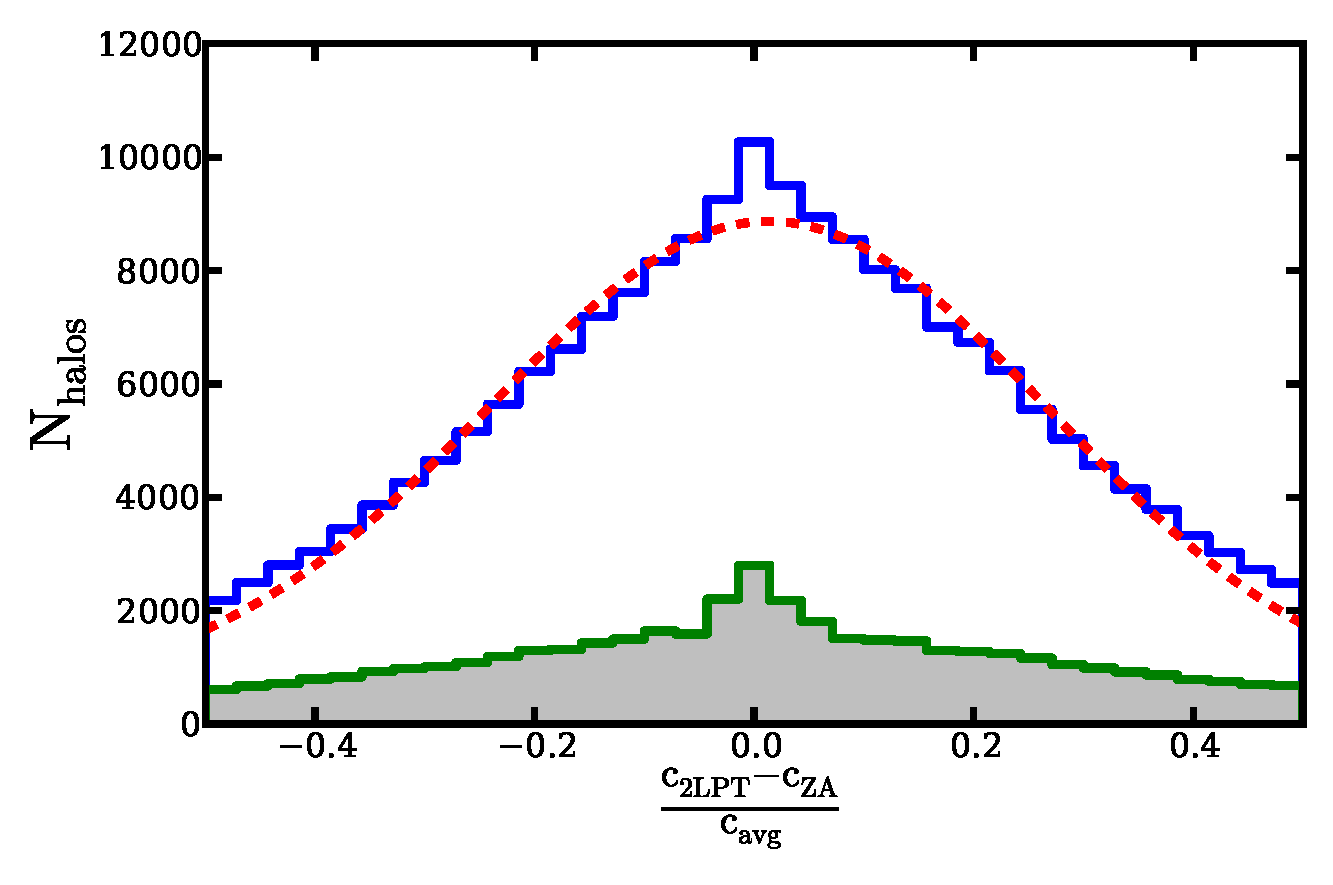
\includegraphics[width=0.48\linewidth]{diff-hist_c_snap061_(0.0-1.0).eps}
	\end{subfigure}
	\caption[Histograms of $\Delta M_{\mathrm{vir}}$ and $\Delta c$]{\footnotesize Like Figure~\ref{fig:diff-hist_Xoff}, but for histograms of $\Delta M_{\mathrm{vir}}$ in the left column and $\Delta c$ in the right column.  Again, the top, middle, and bottom rows correspond to snapshots at $z = 14.7$, $z = 10.3$, and $z = 6.0$, respectively, and generalized normal distributions fit to the data, excluding the central bin, are overplotted with a red dashed line.}
	\label{fig:diff-hist_Mvir_c}
\end{figure*}

We consider $\Delta M_{\mathrm{vir}}$ and $\Delta c$ as a function of average halo mass $M_{\mathrm{vir},\lpt} - M_{\mathrm{vir},\za}$ in Figure~\ref{fig:delta-v-Mavg}.  The data is binned on a 2--D grid with a logarithmic color map for three representative timesteps.  A linear fit to the data is overplotted in red, and a dotted blue line is provided at $\Delta M_{vir} = 0$ and $\Delta c = 0$ to guide the eye.

We find that $\Delta M_{vir}$ tends to increase with increasing $M_{\mathrm{vir,avg}}$, a trend that is, again, most pronounced at high redshift.  \lpt\ halos are consistently more massive than their \za\ counterparts, with the difference increasing with average halo mass.  While less massive halo pairs have a larger spread in the difference in \lpt\ and \za\ mass, more massive halo pairs are more consistently heavier in \lpt\ than in \za.  The slope of the fit line trends towards zero as we progress in redshift, with little average mass dependence by $z = 6$.

The picture is less clear for concentration.  We find a small trend for more massive halo pairs to be more concentrated in \za, but this trend is weaker than for $\Delta M_{\mathrm{vir}}$.  The data have a larger variance than $\Delta M_{\mathrm{vir}}$, and fits have and overall shallower slope.  Mass dependence all but disappears by $z = 6$.

\begin{figure*}[t]
	\centering
	\begin{subfigure}{}
		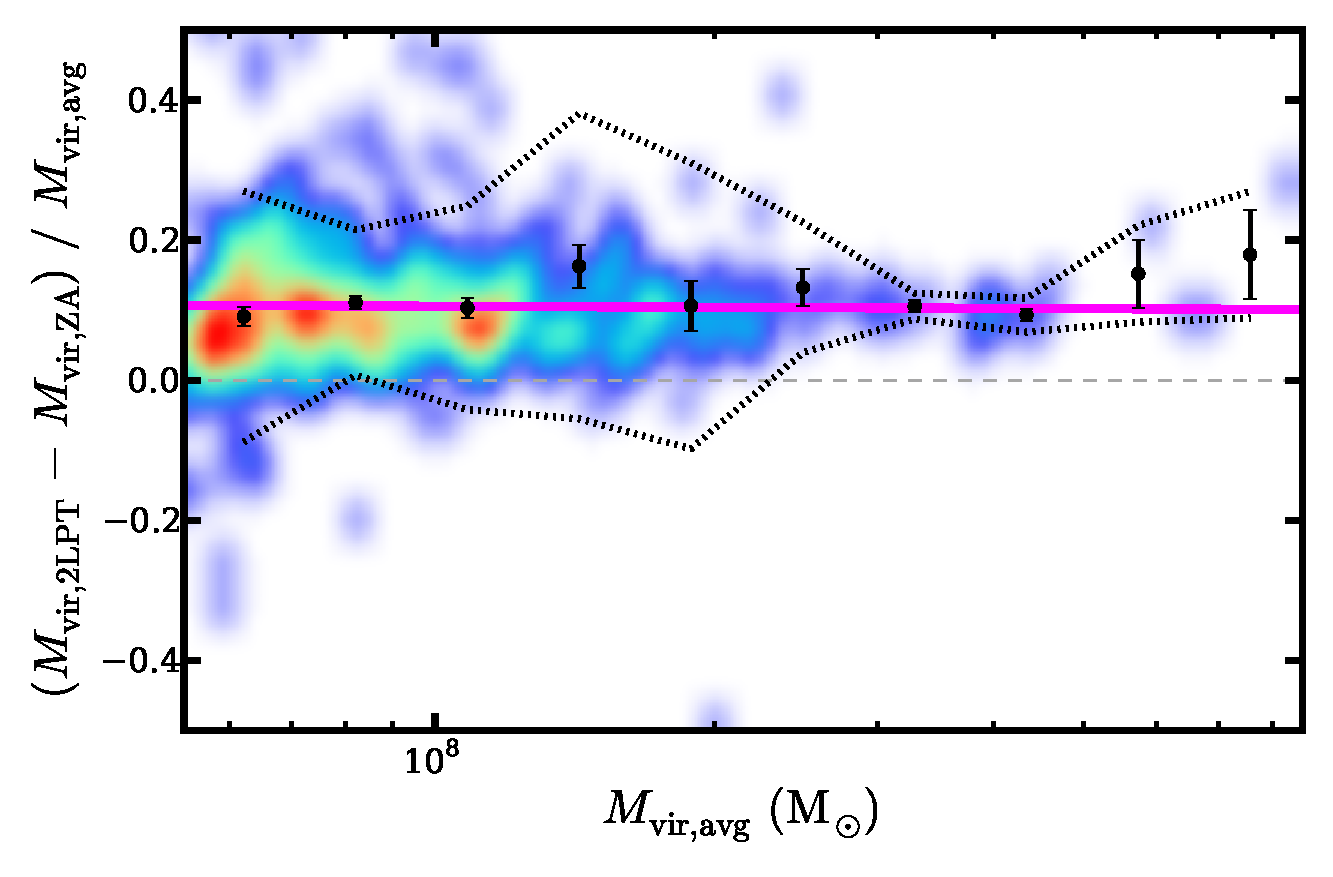
\includegraphics[width=0.48\linewidth]{dM-v-Mavg_snap040.eps}
	\end{subfigure}
	~
	\begin{subfigure}{}
		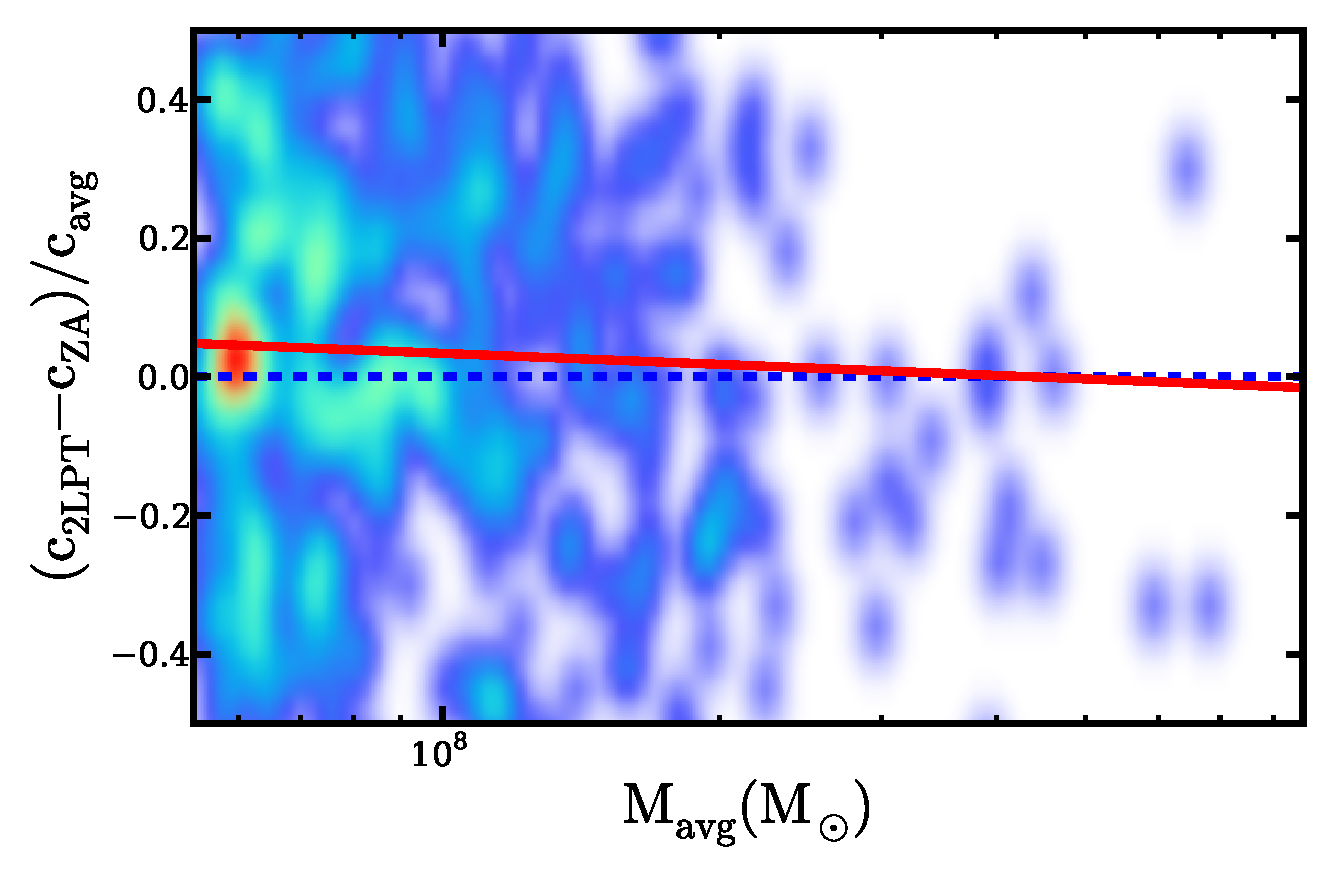
\includegraphics[width=0.48\linewidth]{dc-v-Mavg_snap040.eps}
	\end{subfigure}
	\\
	\begin{subfigure}{}
		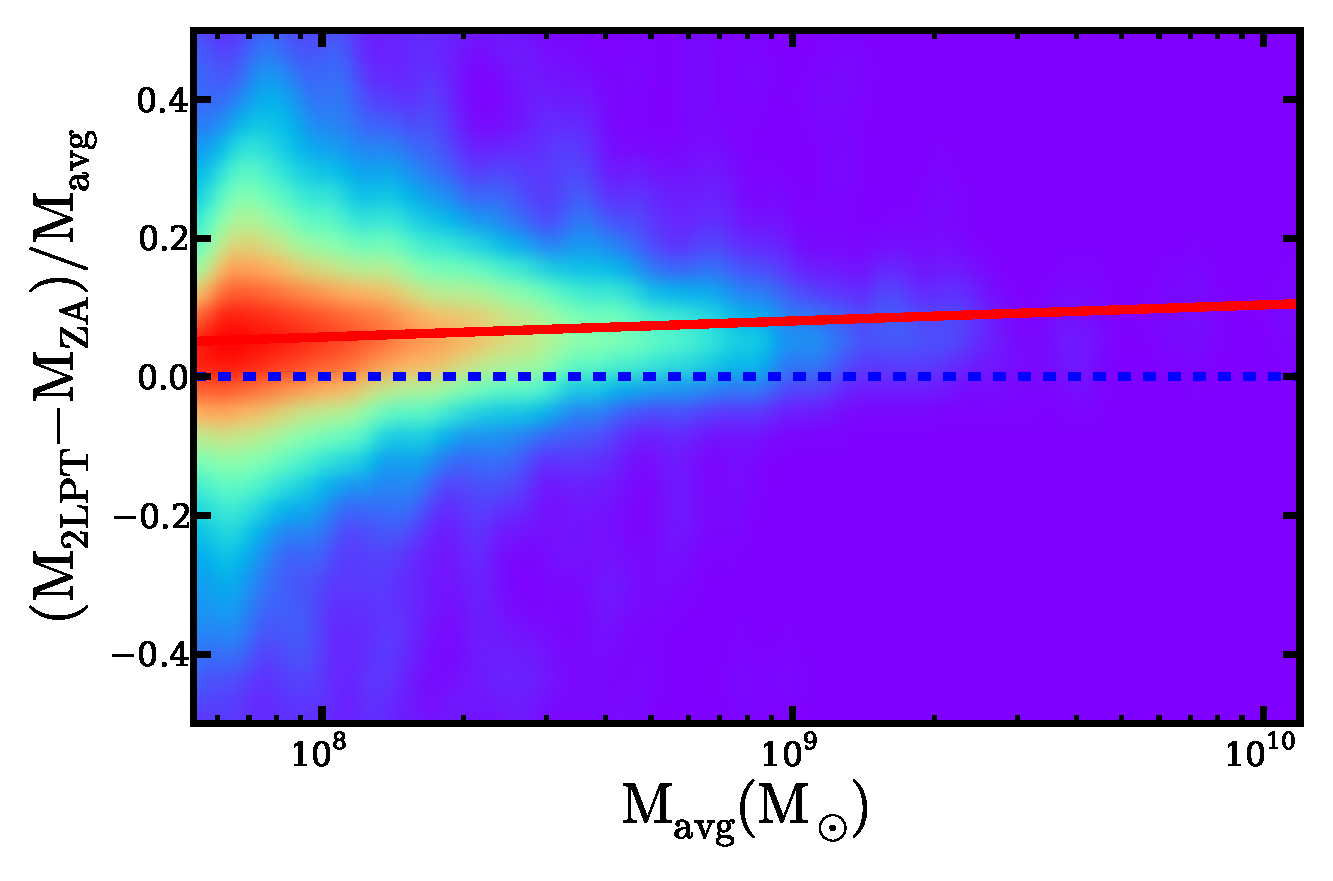
\includegraphics[width=0.48\linewidth]{dM-v-Mavg_snap050.eps}
	\end{subfigure}
	~
	\begin{subfigure}{}
		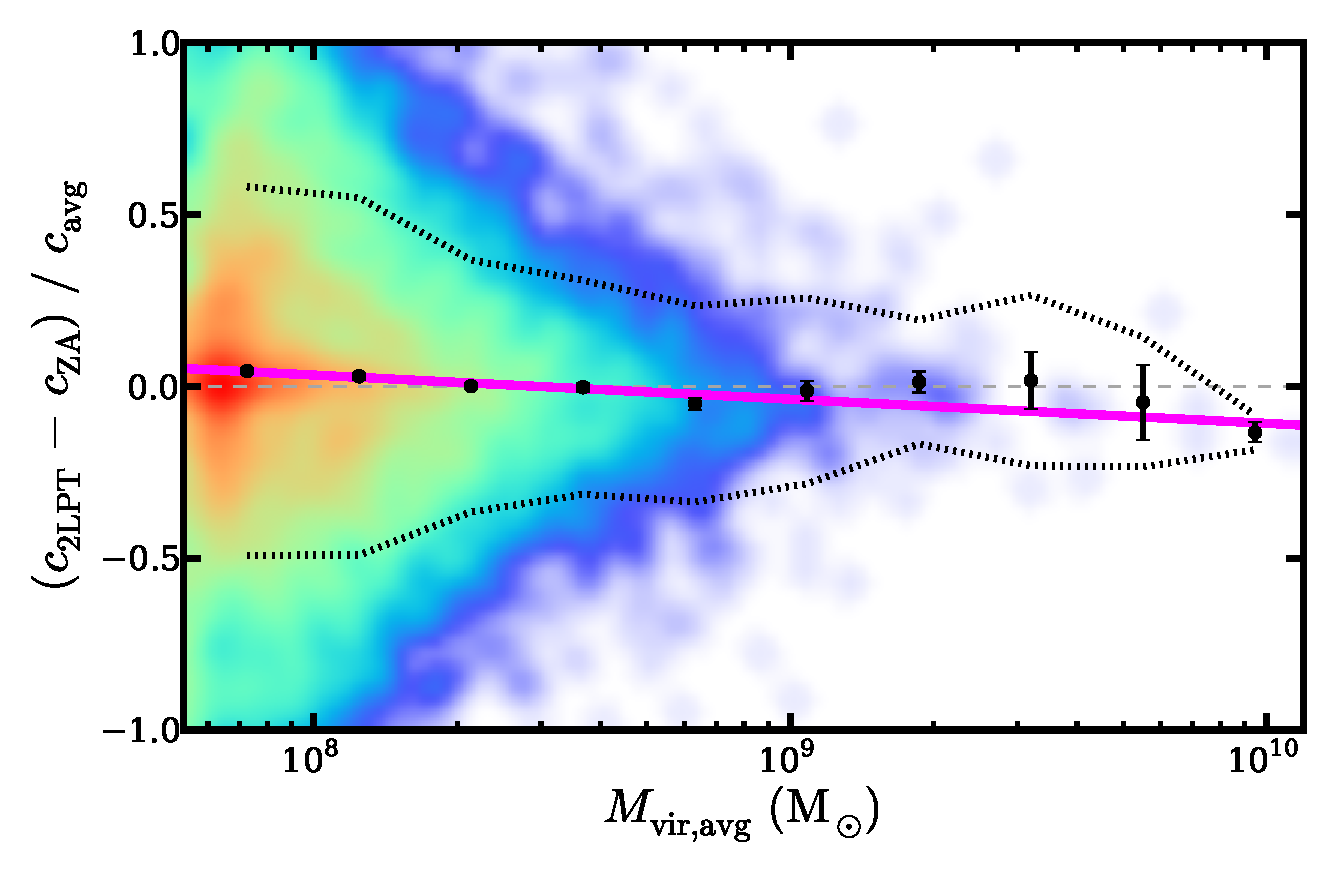
\includegraphics[width=0.48\linewidth]{dc-v-Mavg_snap050.eps}
	\end{subfigure}
	\\
	\begin{subfigure}{}
		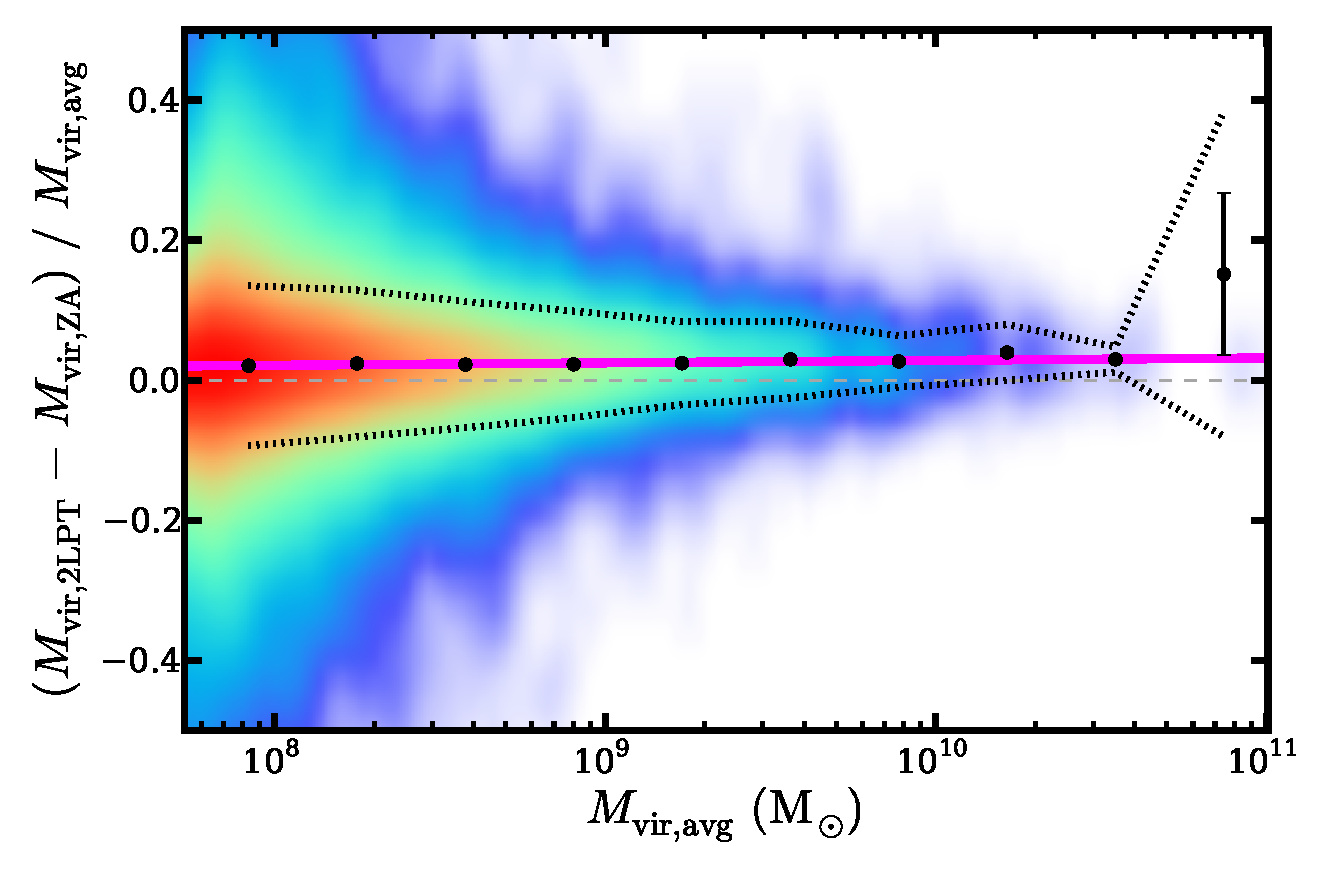
\includegraphics[width=0.48\linewidth]{dM-v-Mavg_snap061.eps}
	\end{subfigure}
	~
	\begin{subfigure}{}
		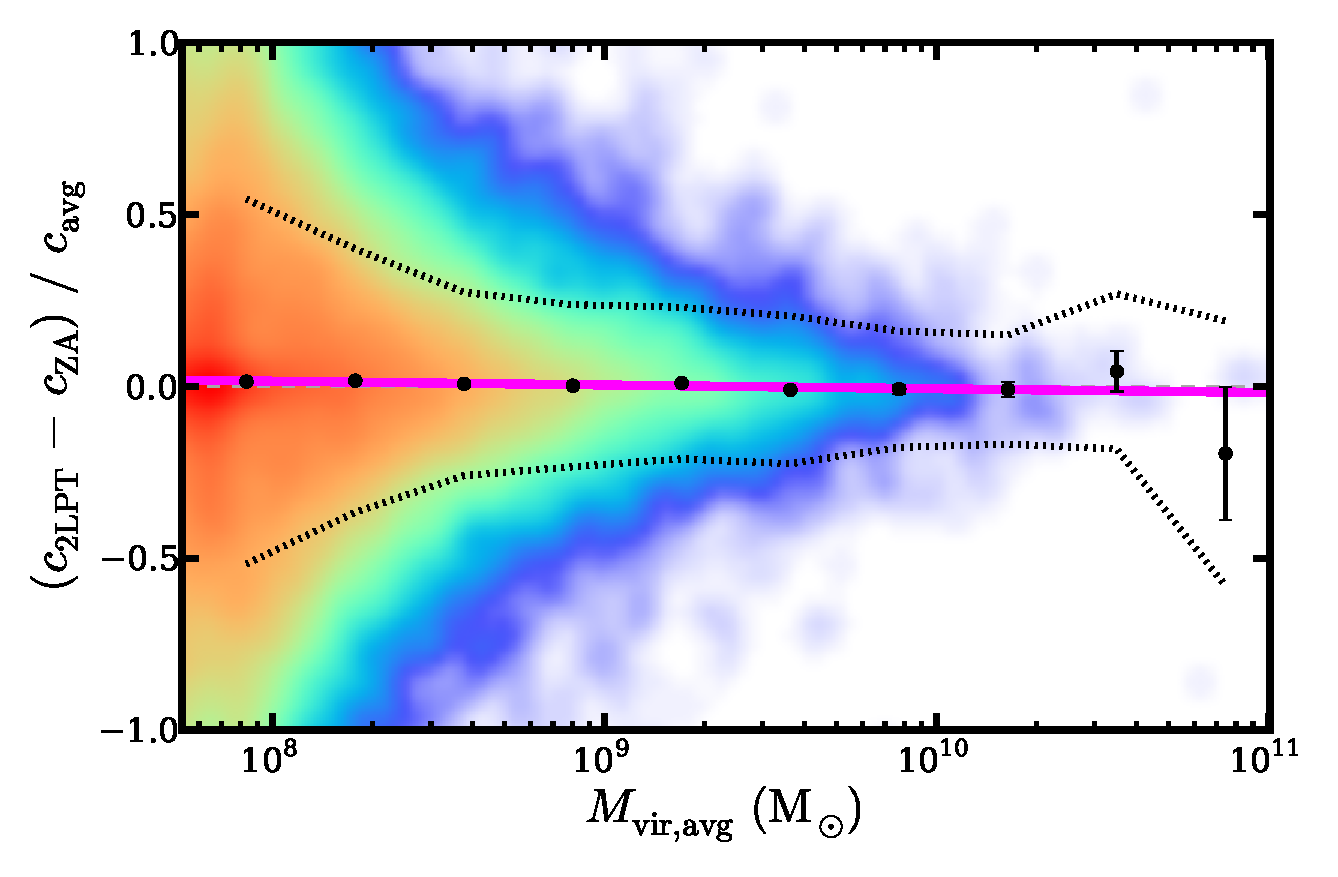
\includegraphics[width=0.48\linewidth]{dc-v-Mavg_snap061.eps}
	\end{subfigure}
	\caption[$\Delta M_{\mathrm{vir}}$ and $\Delta c$ as a function of $M_{\mathrm{vir,avg}}$]{\footnotesize $\Delta M_{\mathrm{vir}}$ (left column) and $\Delta c$ (right column) as a function of $M_{\mathrm{vir,avg}}$.  Halos are counted in 2--D rectangular bins and smoothed with a Gaussian kernel with a logarithmic color scale.  The red line is the least-squares best fit to the data.  The blue dashed line at zero is provided to guide the eye.  The three rows again correspond to snapshots at $z = 14.7$, $z = 10.3$, and $z = 6.0$, respectively.}
	\label{fig:delta-v-Mavg}
\end{figure*}

To more quantitatively assess the time progression of our various trends, see Figure~\ref{fig:fit_trends}, where we plot the mean, standard deviation, skew, and kurtosis of the fitting distributions for $\Delta X_{\mathrm{off}}$, $\Delta M_{\mathrm{vir}}$, and $\Delta c$ as a function of redshift in the left column, and the slopes of the fits for Figure~\ref{fig:delta-v-Mavg} in the right column.  \textcolor{red}{(Talk about fits to fits and trends with redshift here for Figure~\ref{fig:fit_trends}.)}

\begin{figure*}[t]
	\centering
	\begin{subfigure}{}
		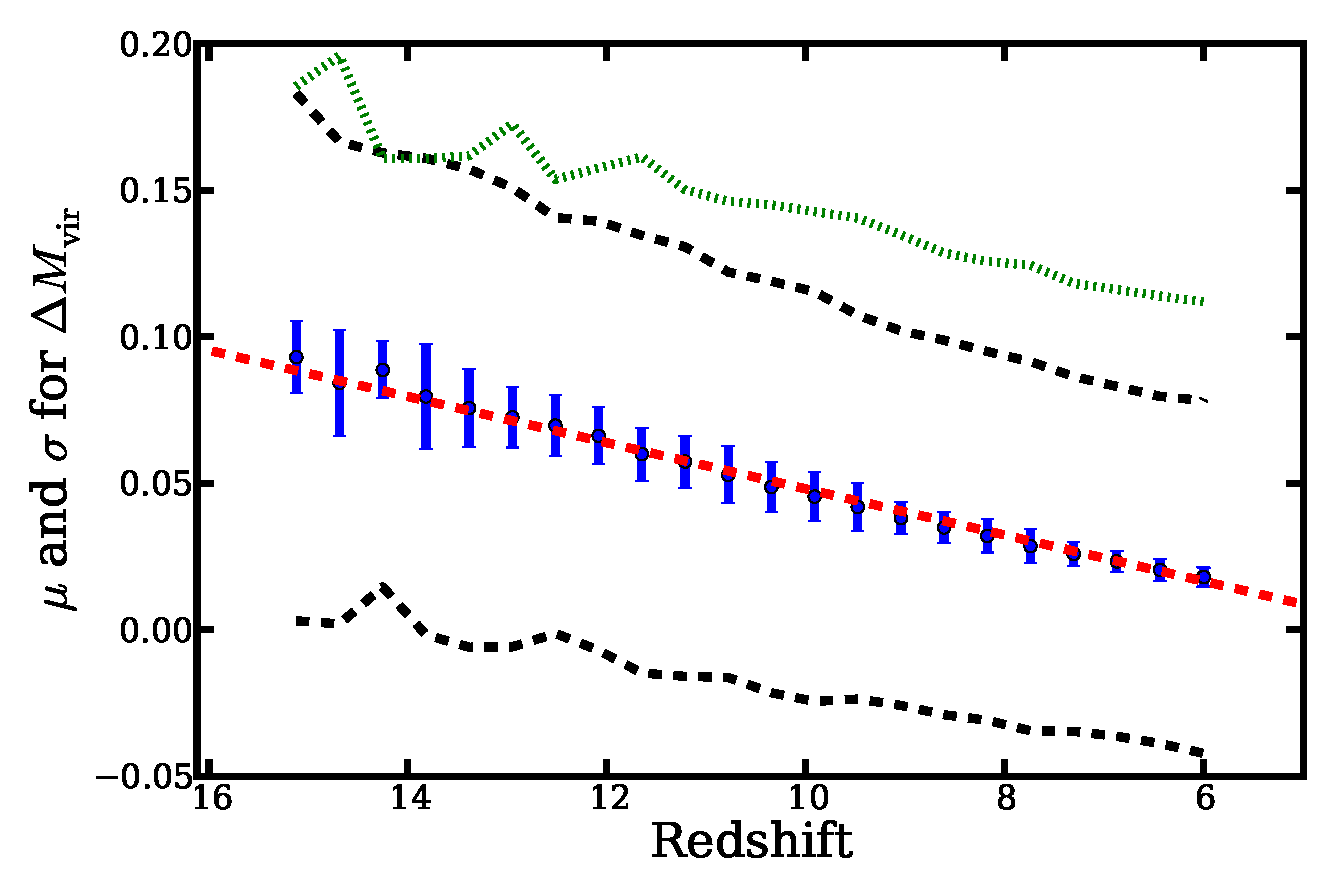
\includegraphics[width=0.48\linewidth]{mean_stdev_Mvir.eps}
	\end{subfigure}
	~
	\begin{subfigure}{}
		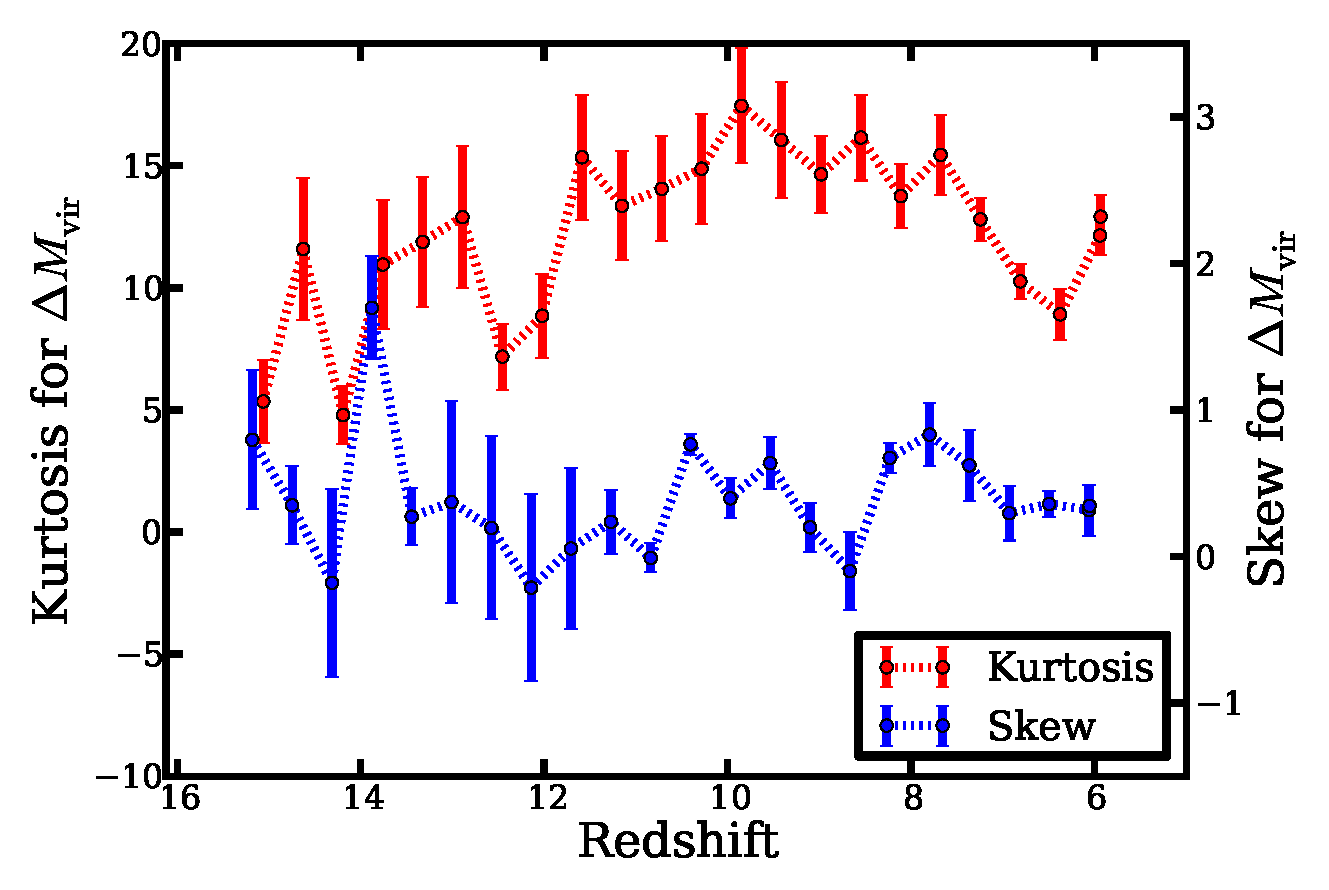
\includegraphics[width=0.48\linewidth]{skew_kurtosis_Mvir.eps}
	\end{subfigure}
	\\
	\begin{subfigure}{}
		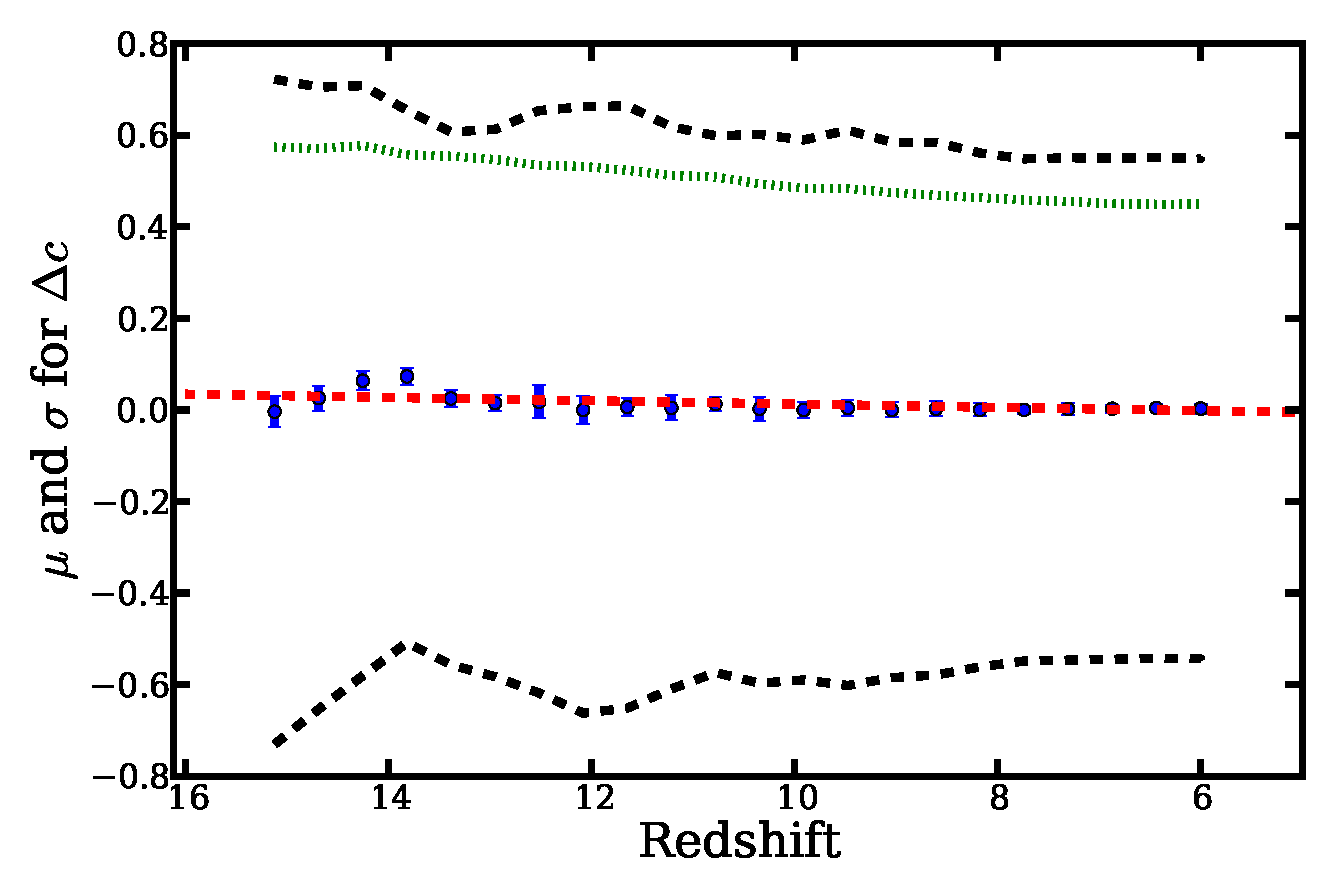
\includegraphics[width=0.48\linewidth]{mean_stdev_c_rockstar.eps}
	\end{subfigure}
	~
	\begin{subfigure}{}
		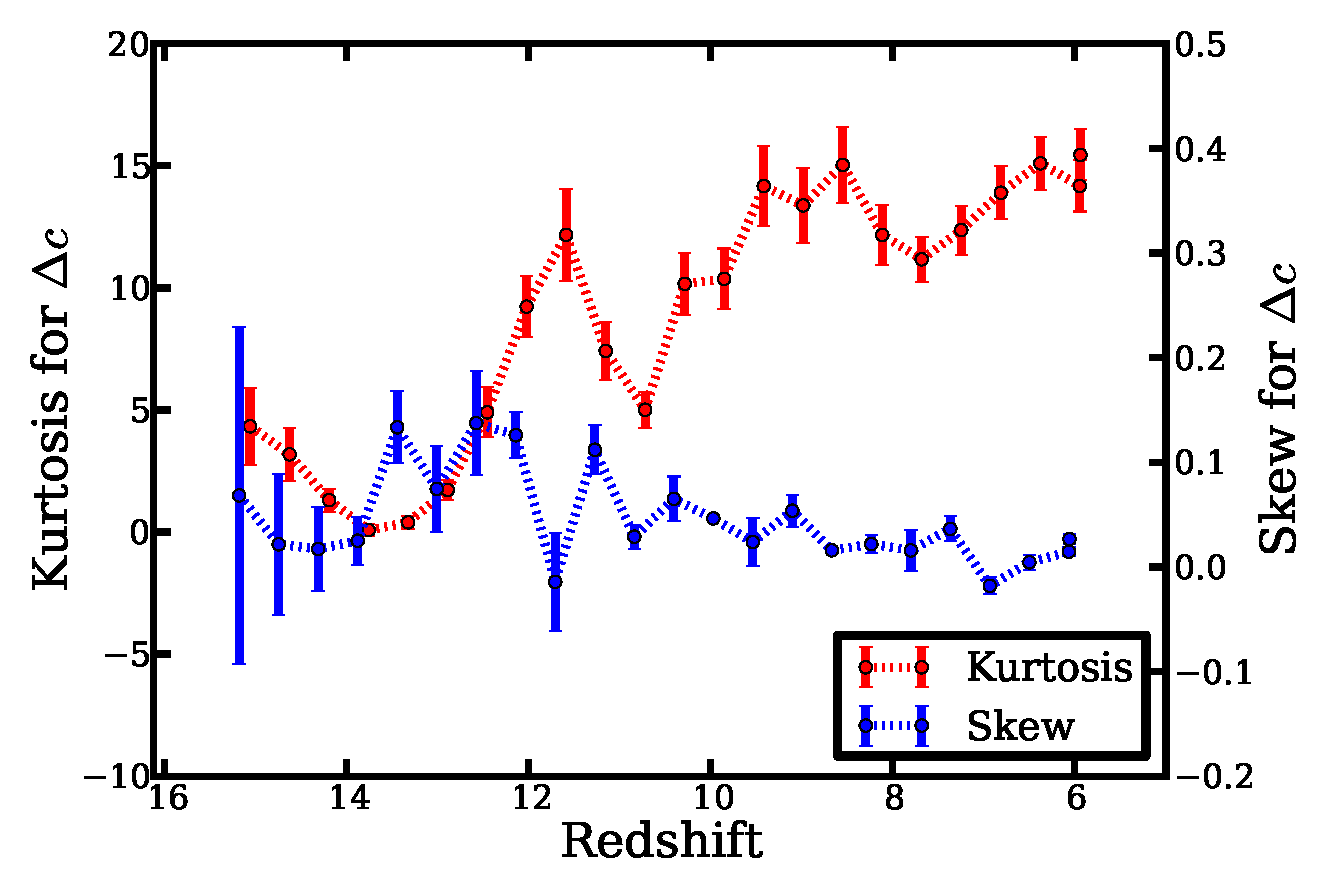
\includegraphics[width=0.48\linewidth]{skew_kurtosis_c_rockstar.eps}
	\end{subfigure}
	\\
	\begin{subfigure}{}
		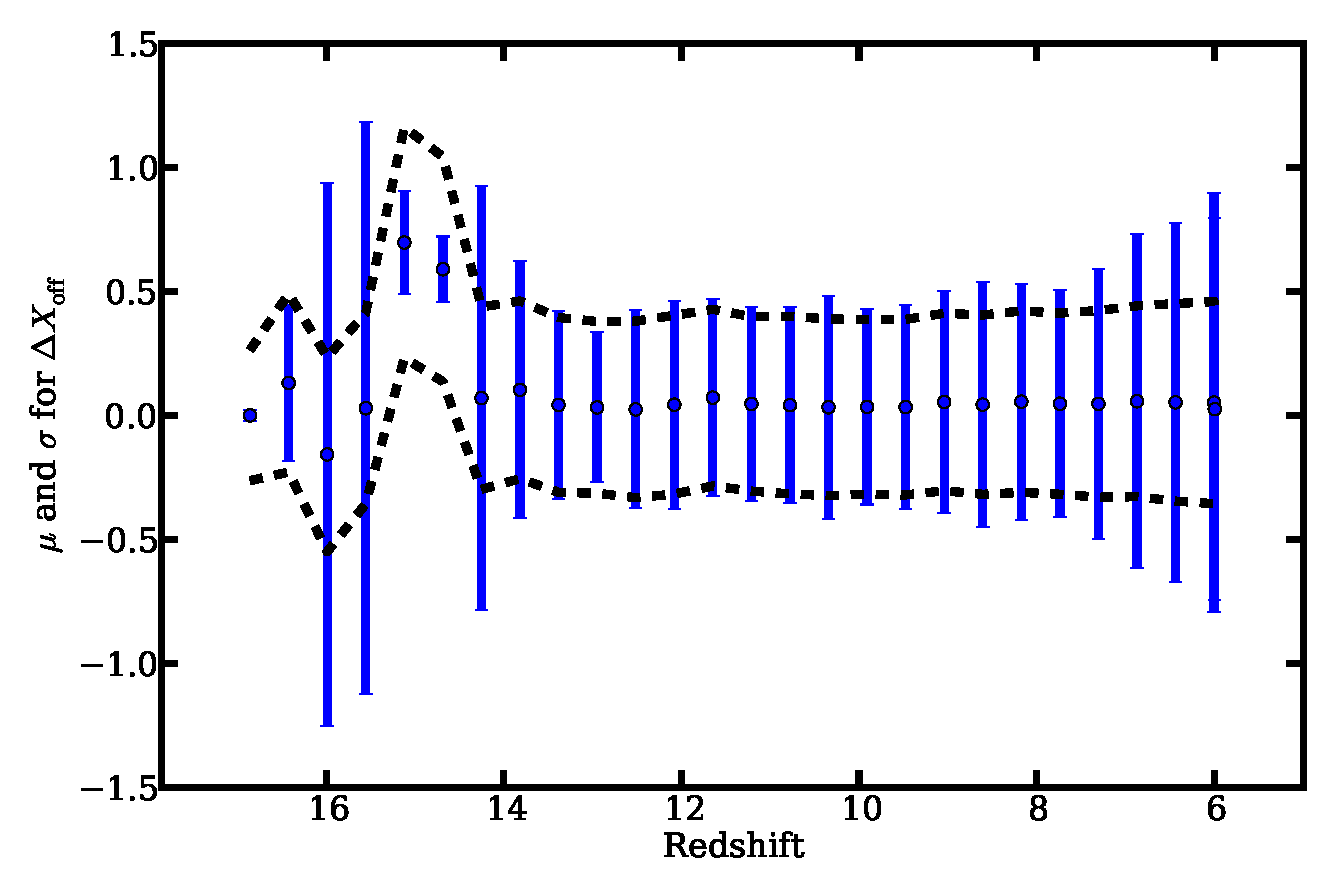
\includegraphics[width=0.48\linewidth]{mean_stdev_Xoff.eps}
	\end{subfigure}
	~
	\begin{subfigure}{}
		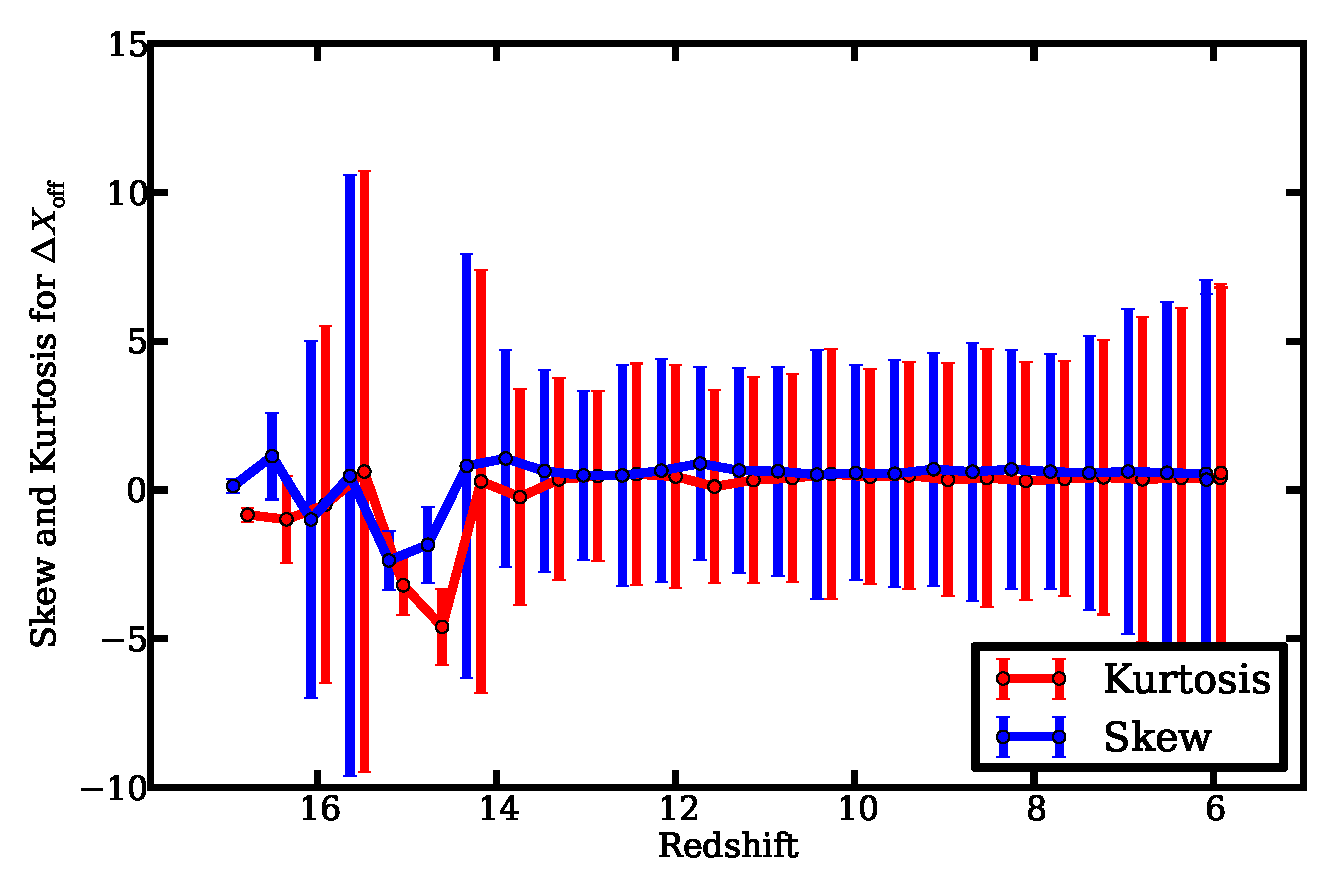
\includegraphics[width=0.48\linewidth]{skew_kurtosis_Xoff.eps}
	\end{subfigure}
	\caption[Statistics for Gaussian fits]{\footnotesize \textcolor{red}{Expand caption.}  \emph{Left column:}  Mean and standard deviation (top panel), and skew and kurtosis (bottom panel) of the generalized normal distribution fits as a function of redshift for histograms in Figure~\ref{fig:diff-hist_Xoff} and Figure~\ref{fig:diff-hist_Mvir_c}.  In the top panel, the points have been offset slightly from each other in redshift to avoid overlap.  \emph{Right column:}  Slope of fits as a function of redshift for $\Delta M_{\mathrm{vir}}$ (top panel) and $\Delta c$ (bottom panel) from Figure~\ref{fig:delta-v-Mavg}.}
	\label{fig:fit_trends}
\end{figure*}

